\documentclass[]{article}

\usepackage[]{geometry}
\geometry{
  top=1in,            % <-- you want to adjust this
  inner=1in,
  outer=1in,
  bottom=1in,
  headheight=3ex,       % <-- and this
  headsep=2ex,          % <-- and this
}
\usepackage[T1]{fontenc}
\usepackage{cmbright}
\usepackage{mathtools}
\usepackage{algorithmic}
\usepackage{fancyhdr}
\usepackage{amssymb}
\usepackage{multicol}
\usepackage{parskip}
\usepackage{titling}
\usepackage{fancyvrb}
\pretitle{\begin{flushleft}\LARGE\sffamily}
\posttitle{\par\end{flushleft}\vskip 0.5em}
\preauthor{\begin{flushleft}}
\postauthor{\par\end{flushleft}}
\predate{\begin{flushleft}\scshape}
\postdate{\par\end{flushleft}}
\setlength{\droptitle}{-20pt}
\setlength{\headheight}{15.2pt}
\pagestyle{fancy}

\setcounter{secnumdepth}{1}

\fancyhf{}
\renewcommand{\headrulewidth}{0pt} % remove line at top
\lhead{\fancyplain{}{CS 4780 A3}}
\rhead{\fancyplain{}{Justin Cheng \emph{jc882}, Sunling Selena Yang}}
\rfoot{\fancyplain{}{\thepage}}

\begin{document}

\title{CS 4780 Assignment 3}
\author{Justin Cheng and Sunling Selena Yang}
\date{\today}
\maketitle

\hrule
\vskip 1em

\section{Perceptron and SVM}
\subsection{a.}
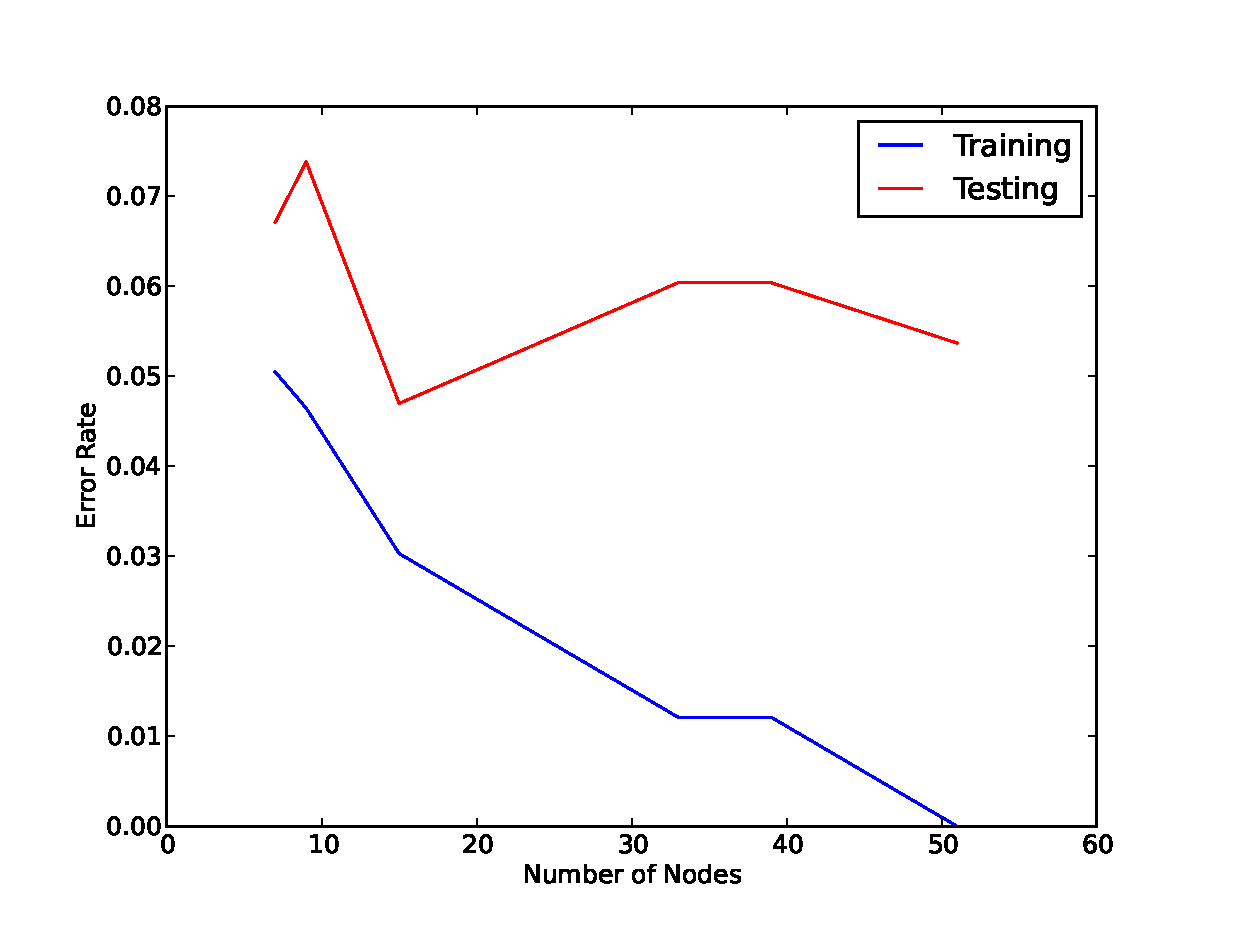
\includegraphics[scale=0.5]{data/images/part_a.eps}

The training error decreases dramatically after the first few iterations, although it is not strictly decreasing. However, after the 15th iteration the training error is 0, meaning that a separating hyperplane was learnt.

The validation error fluctuates wildly for the first few iterations, but then stabilizes at about 0.217.

This does appear to confirm the fact that the Perceptron algorithm converges after a finite number of iterations.

Prefer a lower learning rate for improved accuracy, though over a longer number of iterations. If the learning rate is too high, over-correction is likely to occur and you might end up oscillating around the true separating hyperplane.

We should not use the dual algorithm, since it stores needless information and requires us to keep the whole training set in memory, even when we perform predictions. If we don't care about the $\alpha$s, we can simply use the primal algorithm to update $w_k$ incrementally. (TODO how about accuracy?)

\subsection{b.}
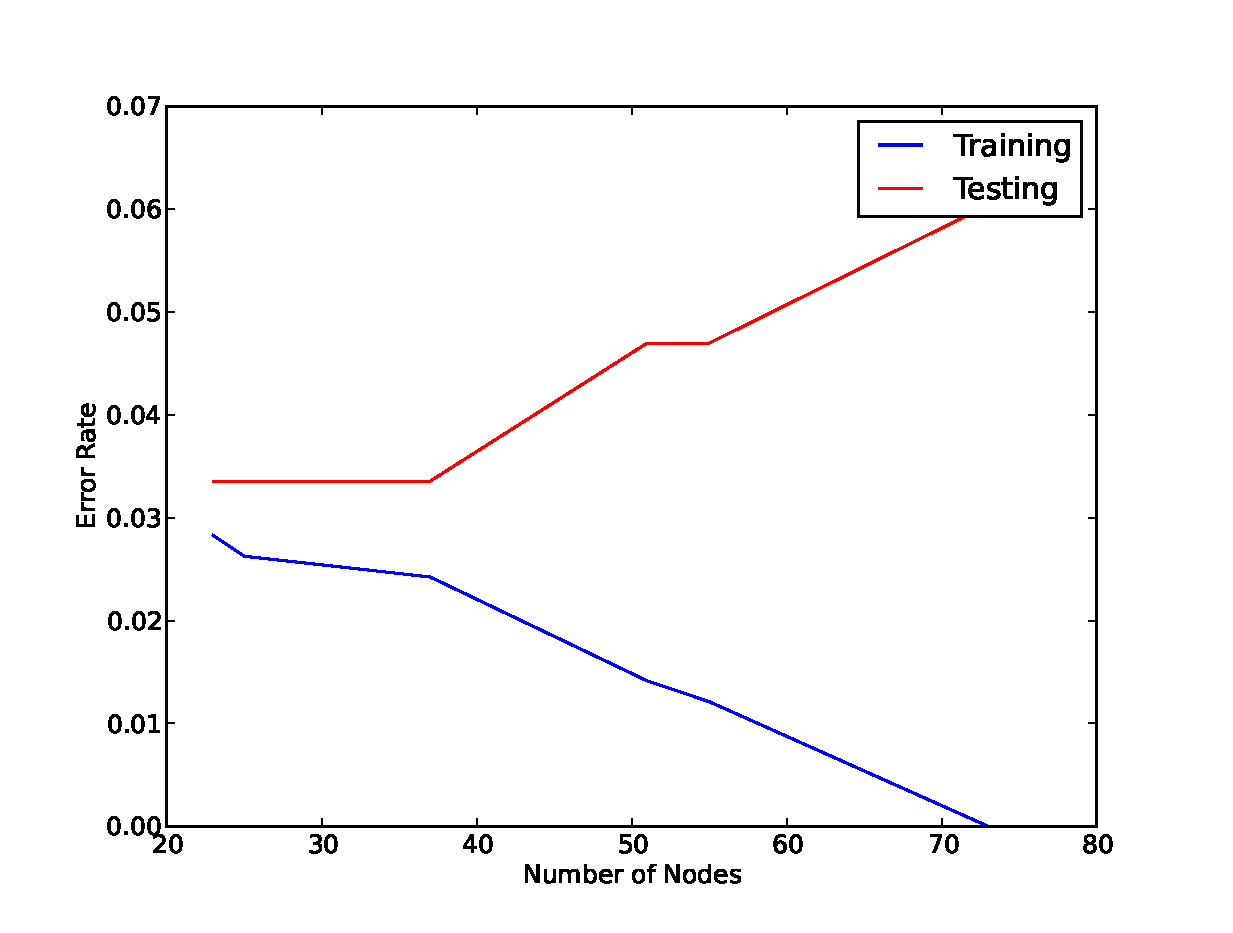
\includegraphics[scale=0.5]{data/images/part_b.eps}

The smallest validation error rate is achieved at $C = 8$. (TODO compare to (a)).

The training error rate goes to 0 as C increases, but the validation error steadily decreases to a minimum at $C=8$, and increases after that. (TODO Why?)

\subsection{c.}
\includegraphics[scale=0.42]{data/images/part_c_tra.eps}
\includegraphics[scale=0.42]{data/images/part_c_val.eps}
The graph on the left shows the training error, and the graph on the right shows the validation error. Perceptron works badly on reorder-3 because in that reordering, all the positive examples come before the negative examples. Thus, the algorithm makes very few updates in each iteration (at most 4), since after the first mistake on the first positive example, all examples are classified correctly until the first negative example, and then after a couple of corrections, all subsequent examples (all negative) are all classified correctly. Thus, the hypothesis learned is not indicative of a true weighing of all the features.

Using $SVM_{light}$ with $C=8$, the training error in all cases is 0.009, and the validation error in all cases is 0.205. 

\subsection{d.}
Let $H_1$ be the hypothesis produced by the perceptron algorithm. Let $H_2$ be the hypothesis produced by SVM. Let $d_i$ be the \# of examples $H_i$ makes an error on, but not $H_{i'}$, $i' \neq i$.

$d_1 = 49$

$d_2 = 37$

$k = d_1 + d_2 = 86$

If $Err_p(h_1) = Err_p(h_2)$, then $d_1$, $d_2$ are binomially distributed with $p = \frac{1}{2}$.

Null hypothesis: $D_1$ is binomial with $p=\frac{1}{2}$ and $k=86$.

$P(D_1 \ge d_1~|~p = 0.5, k) = 0.080 > 0.025$

Do not reject null hypothesis. The Linear SVM has a prediction error that isn't significantly different.

(TODO: So...?)

\section{Linear Separability}
\subsection{a.}
Consider the construction where each sample with an unknown feature is assigned $k$ for exactly one of $t_{i1},...,t_{im}$, by the problem definition. Thus, for each of these $m$ samples, exactly one of these $t$ variables is set to $k$. We can then classify each of these samples using only the value of that indicator feature.

\subsubsection{Example}
Consider $x_1 = (1,?)$, $x_2 = (1,2)$, $x_3 = (1,1)$, with $y_1 = -1, y_2 = -1, y_3 = +1$. These examples are obviously not separable in $\mathbb{R}^2$ if we set the unknown feature to 0. In this example, $m=1$, so we add 1 indicator variable, setting it to $k=1$ for $x_1$ and $0$ for all other samples, so that $x_1 = (1,0,1)$, $x_2 = (1,2,0)$, $x_3 = (1,1,0)$.

After running Perceptron, we get $w = (0,1,-1)$, which separates all the examples correctly.

In fact, for any $m$, and for any $k$, you can set $w_{t_{ii}}$, for $0 \le i \le m$ to have an absolute value greater than the sum of all other non-$t_{ij}$ terms, and set its sign accordingly based on $y_i$, to ensure that sample $i$ is classified correctly. You do not need to care about the other $t_{ij}$, since these are 0 everywhere else and will not affect the computation other than for that specific sample.

\subsection{b.}
The radius of $\tilde S$ is simply $\max \{R,k\}$, and since $\delta$ is arbitrarily defined, it remains the same. Using the same derivation as in lecture, replace $x_i^2 \le R^2$ with $x_i^2 \le (\max \{R, k\})^2$.

The upper bound on the number of mistakes made is thus $\frac{(\max \{R,k\})^2}{\delta^2}$.

\section{Linear SVM}

\subsection{a.}
???

\subsection{b.}
For the hard margin unbiased SVM, the dual QP is

\begin{align*}
\max\quad & D(\alpha) = \sum_{i=1}^n \alpha_i - \frac{1}{2} \sum_{i=1}^n \sum_{j=1}^n y_iy_j\alpha_i\alpha_j(x_i \cdot x_j)\\
\text{s.t.}\quad & 0 \le \alpha_i
\end{align*}

Since $x_i^Tx_j = 0$ for $i \neq j$, the objective function simplifies to $\max \sum_i \alpha_i - \frac{1}{2}\sum_{i=1}^n \alpha_i^2 l_i$, since $y_iy_i = 1~\forall i$.

Further simplifying, we get $\max \sum_i \left( \alpha_i (1-\frac{1}{2}\alpha_i l_i)\right)$, but this is simply a sum of quadratic terms each in $\alpha_i$, and to maximize this, we can set $\alpha_i = \frac{1}{l_i}$.

This is also the dual variable $\alpha_i$ for each training example $(x_i, y_i$)

\subsection{c.}
First, note that in the perceptron primal algorithm, for each update, you add $y_i x_i$ to $w_k$. If all $x_i$ are scaled up, such that $x_i^\star = kx_i$, in each update, you will instead add $ky_ix_i$ to $w_k$. Thus, after normalizing, $w$ will still be the same as before, since we simply multiplied $w$ (unnormalized) by $k$.

Now, the error $\xi_i$ will be multiplied by $k$ for each $i$. To see why this is the case, notice that this value depends on the distance to the hyperplane, $w^Tx_i$. In the new case, this value is now $w^Tx_i^\star = kw^Tx_i$, so that this distance is multiplied by $k$.

Thus, in our objective, we want to set $C$ such that our new objective $\min \frac{1}{2}||w^{\star 2}|| + C^\star \sum_{i=1}^n \xi_i^\star$ is a constant factor of our original objective function.
But we found out the new values of $w$ and $xi$, so we know our new objective is equivalently $\min \frac{1}{2}||w^2|| + C^\star \sum_{i=1}^n k\xi_i$. Comparing terms, $kC^\star = C \Rightarrow C^\star = \frac{C}{k}$.

Thus, $C$ should be divided by $k$ so that the new solution defines the same linear classifier.

The resulting $(w^\star, \xi^\star)$ is equivalently $(w, k\xi)$. 

\end{document}